\subsection{\large{\textit{cF}8-C (Inverse)}}\vspace{-0.1in}
Inverse Diamond


\begin{figure}[H]
\begin{minipage}{0.34\textwidth}\centering
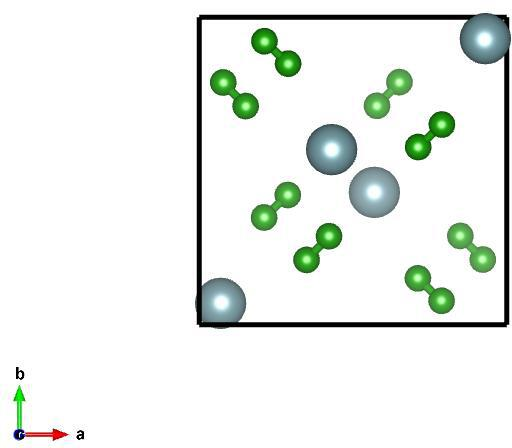
\includegraphics[width=0.9\linewidth,height=2in,keepaspectratio]{/Users/rosecers/work_folders/structures_for_photonics/reference/ref_inp/workspace/bef316054c4336e6d792adceae8ce288/final_images/analog_trim.jpg}\\
\small{Image of \textit{cF}8-C, generated by Vesta}
\end{minipage}\hfill
\begin{minipage}{0.65\textwidth}\raggedright
{\setlength{\mathindent}{0cm}
\begin{equation*}
\begin{split}&\boldsymbol{a_1} = 1/\sqrt{2}\ \hat{y} + 1/\sqrt{2}\ \hat{z}\\[-8pt]
&\boldsymbol{a_2} = 1/\sqrt{2}\ \hat{x} + 1/\sqrt{2}\ \hat{z}\\[-8pt]
&\boldsymbol{a_3} = 1/\sqrt{2}\ \hat{x} + 1/\sqrt{2}\ \hat{y}
\end{split}
\end{equation*}}

\textbf{Space Group:}	227\hspace{0.5in}\textbf{Point Group:}	$m\bar{3}m$\\
\textbf{Inorganic Crystallographic Database} \#52054\\
\textbf{Structure DOI: }\url{10.1107/S0108768195010810}

\textbf{Photonics DOI: }\url{10.1103/PhysRevLett.65.3152}
\end{minipage}\hfill
\end{figure}
\vspace{-0.25in}


\begin{figure}[H]
\begin{minipage}{0.9\textwidth}\centering
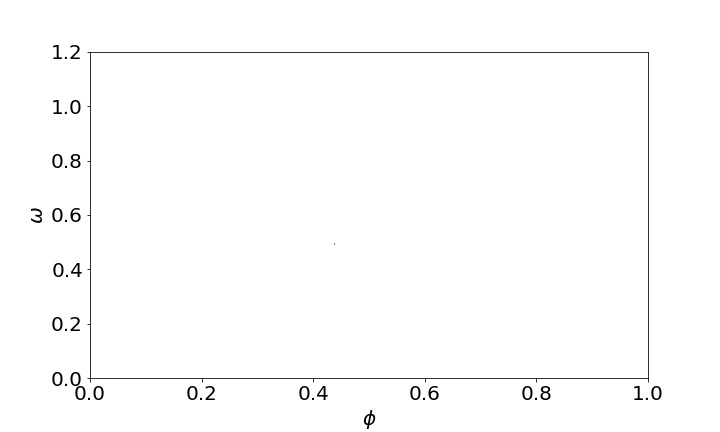
\includegraphics[width=0.9\linewidth,height=2.5in,keepaspectratio]{/Users/rosecers/work_folders/structures_for_photonics/reference/ref_inp/workspace/bef316054c4336e6d792adceae8ce288/final_images/gap_atlas.jpg}
\\
\end{minipage}\hfill\caption{Gap Atlas across filling fraction $\phi$ and frequency $\omega$}
\end{figure}


\begin{figure}[H]
\begin{minipage}{0.5\textwidth}\centering
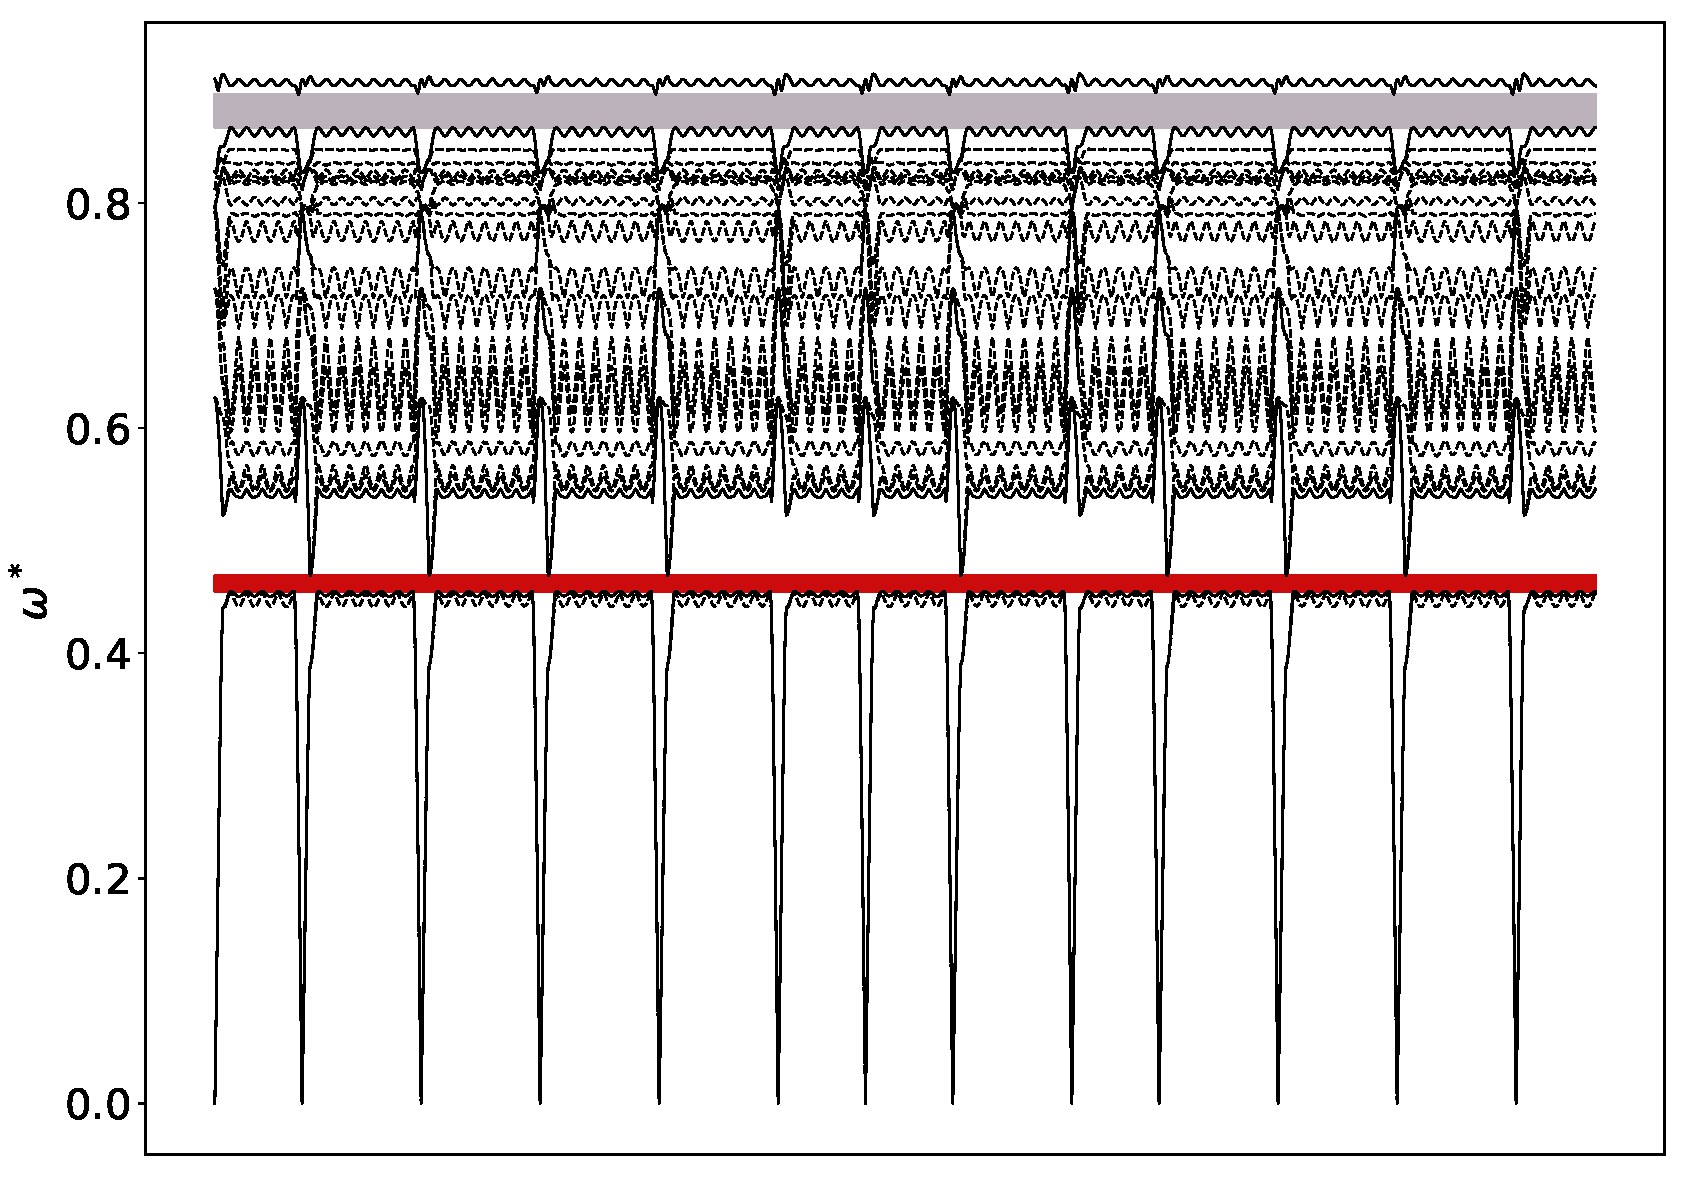
\includegraphics[width=0.9\linewidth,height=2.0in,keepaspectratio]{/Users/rosecers/work_folders/structures_for_photonics/reference/ref_inp/workspace/bef316054c4336e6d792adceae8ce288/./final_images/band_diagram_b=2.pdf}
\\Band Structure across 1st BZ
\end{minipage}\hfill
\begin{minipage}{0.48\textwidth}\centering
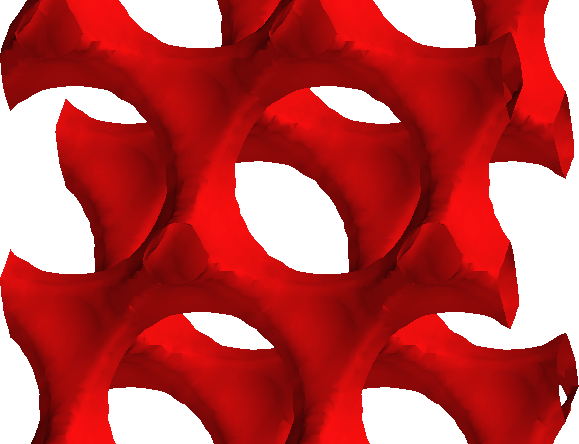
\includegraphics[width=0.9\linewidth,height=2.0in,keepaspectratio]{/Users/rosecers/work_folders/structures_for_photonics/reference/ref_inp/workspace/bef316054c4336e6d792adceae8ce288/final_images/cF8-C_r@gap_2-3.png}
\\View along $a_1$ 
\end{minipage}\hfill\caption{Band Structure and Isosurface of \textit{cF}8-C (Inverse) at radius = 0.47, filling fraction = 0.167, where the largest gap between bands 2 and 3 occurs with gap size 33.84\%.}

\end{figure}
\vspace{-0.25in}


\begin{figure}[H]
\begin{minipage}{0.5\textwidth}\centering
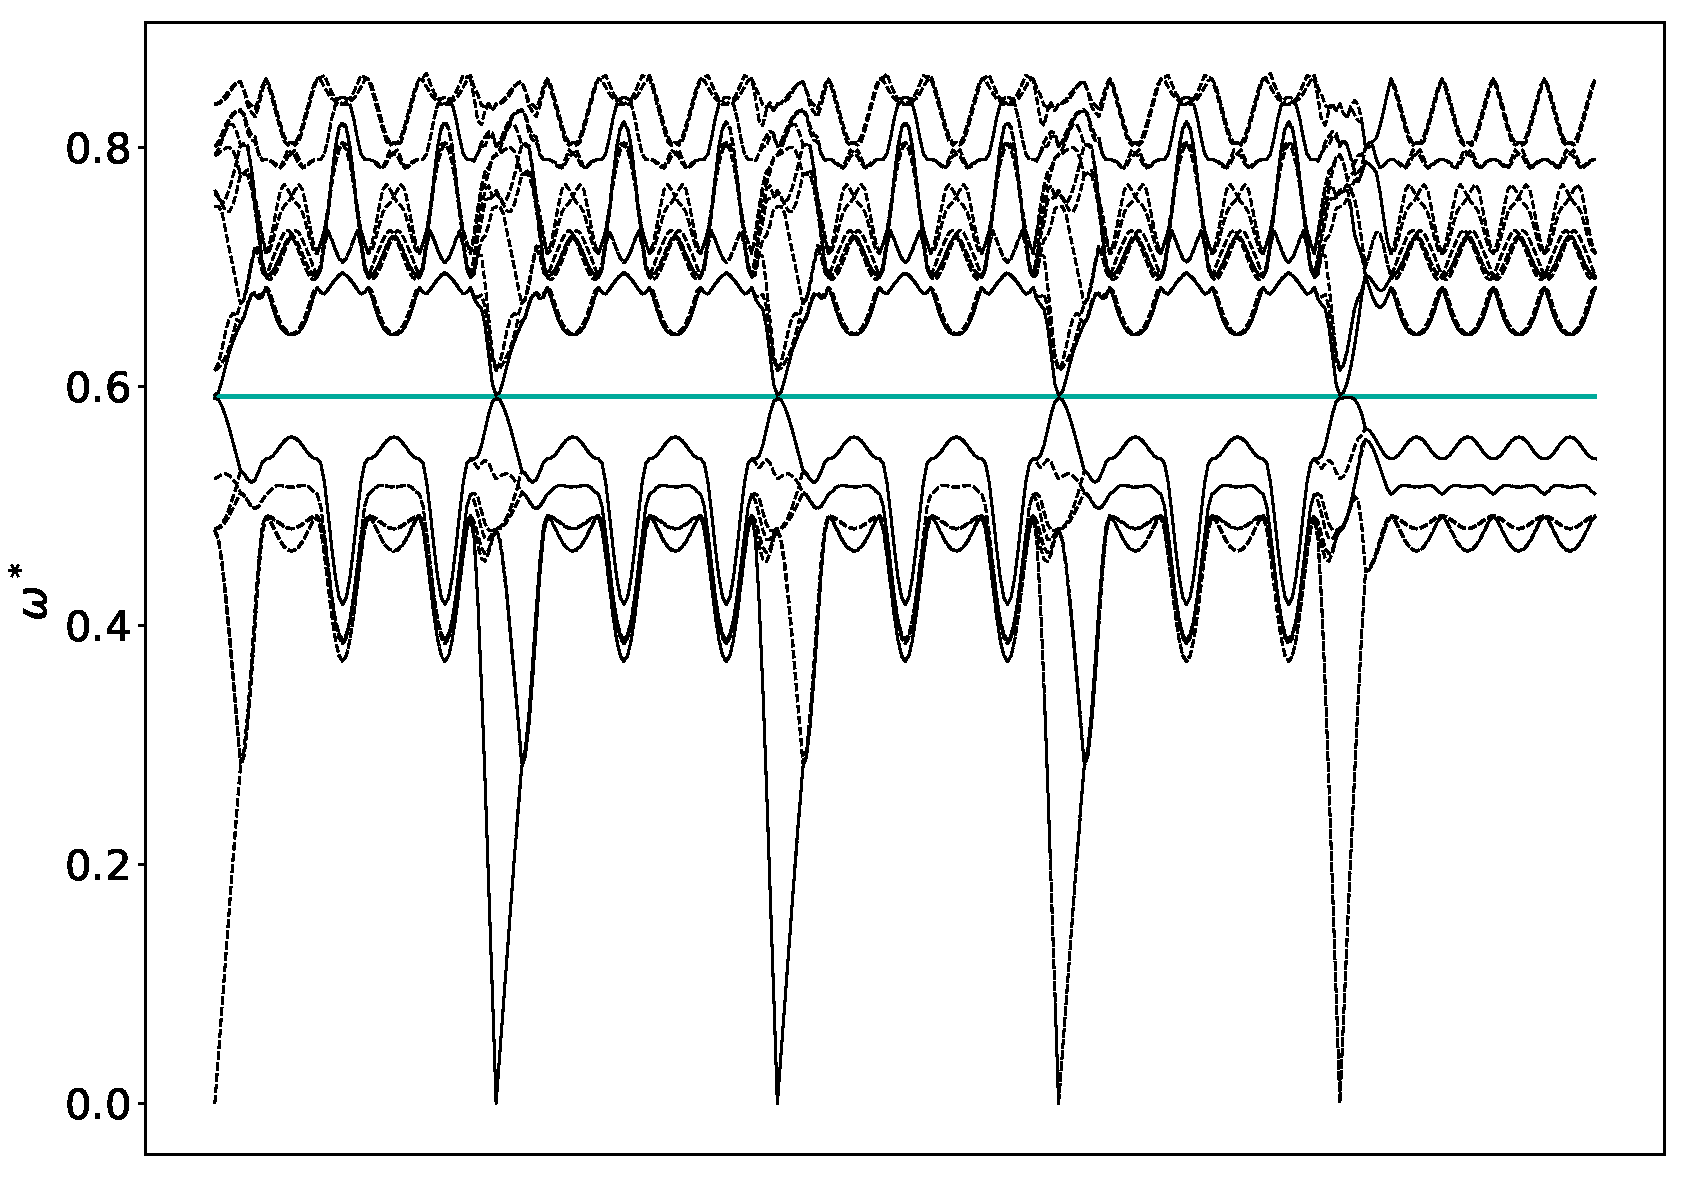
\includegraphics[width=0.9\linewidth,height=2.0in,keepaspectratio]{/Users/rosecers/work_folders/structures_for_photonics/reference/ref_inp/workspace/bef316054c4336e6d792adceae8ce288/./final_images/band_diagram_b=8.pdf}
\\Band Structure across 1st BZ
\end{minipage}\hfill
\begin{minipage}{0.48\textwidth}\centering
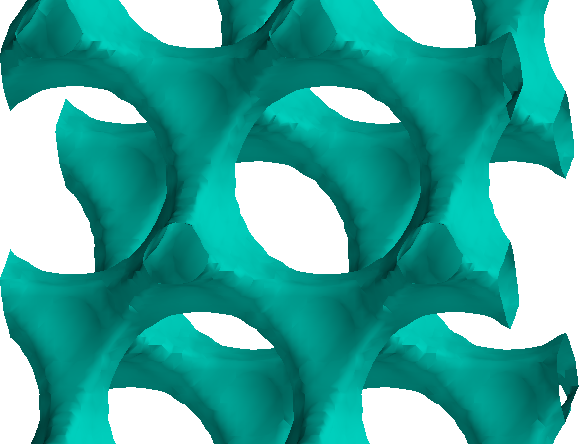
\includegraphics[width=0.9\linewidth,height=2.0in,keepaspectratio]{/Users/rosecers/work_folders/structures_for_photonics/reference/ref_inp/workspace/bef316054c4336e6d792adceae8ce288/final_images/cF8-C_r@gap_8-9.png}
\\View along $a_1$ 
\end{minipage}\hfill\caption{Band Structure and Isosurface of \textit{cF}8-C (Inverse) at radius = 0.47, filling fraction = 0.167, where the largest gap between bands 8 and 9 occurs with gap size 0.19\%.}

\end{figure}
\vspace{-0.25in}

